% $Header$

\documentclass{beamer}

% This file is a solution template for:

% - Giving a talk on some subject.
% - The talk is between 15min and 45min long.
% - Style is ornate.



% Copyright 2004 by Till Tantau <tantau@users.sourceforge.net>.
%
% In principle, this file can be redistributed and/or modified under
% the terms of the GNU Public License, version 2.
%
% However, this file is supposed to be a template to be modified
% for your own needs. For this reason, if you use this file as a
% template and not specifically distribute it as part of a another
% package/program, I grant the extra permission to freely copy and
% modify this file as you see fit and even to delete this copyright
% notice. 


\mode<presentation>
{
  %\usetheme{Warsaw}
  %\usetheme{Berlin}
  %\usetheme{metropolis}
  \usetheme{PaloAlto}
  %\usetheme{CambridgeUS}
  %\usetheme{Berkeley}
  
  % font themes
  \usefonttheme{serif}
  %\usefonttheme{structurebold}

  % color themes
  %\usecolortheme{albatross}
  %\usecolortheme{beetle}
  %\usecolortheme{crane}
  %\usecolortheme{dove}
  %\usecolortheme{fly}
  %\usecolortheme{monarca}
  %\usecolortheme{seagull}
  %\usecolortheme{beaver}
  % color themes
  % or ...

  %\setbeamercovered{transparent}
  \setbeamercovered{transparent=5}
  % or whatever (possibly just delete it)
}


\usepackage[english]{babel}
% Place figures exactly where you mean to
%https://tex.stackexchange.com/a/8633/64425
\usepackage{float}
% Place figures exactly where you mean to
% or whatever

\usepackage[utf8]{inputenc}
% or whatever

\usepackage[T1]{fontenc}
% Or whatever. Note that the encoding and the font should match. If T1
% does not look nice, try deleting the line with the fontenc.

% math
\usepackage{amsmath}
\usepackage{amssymb}
\usepackage{amsthm}
\theoremstyle{definition}
\newtheorem{hyperrule}{Hyperreal Computation Rule}
% math

% tikz
\usepackage{tikz}
\usetikzlibrary{arrows.meta}
\usetikzlibrary{calc}
% tikz
\usepackage{caption}
\usepackage{hyperref}
\hypersetup{
    colorlinks,
    linkcolor={magenta!50!black},
    citecolor={blue!50!black},
    urlcolor={blue!80!black}
}
% large commented sections
\usepackage{comment}
% large commented sections

% some beautiful fonts
\usepackage{yfonts}
% some beautiful fonts

% canceling in equations
\usepackage{cancel}
% canceling in equations

% use alphabetical order for enumeration
%\usepackage{enumitem}
% use alphabetical order for enumeration

\title[Infinitesimal Calculus] % (optional, use only with long paper titles)
{Elementary Calculus--An Infinitesimal Approach, Chapters 01, 02}

\subtitle
{Calculus Based on Nonstandard Analysis} % (optional)

\author[JK,KM] % (optional, use only with lots of authors)
{Jerome Keisler\inst{1}}
% - Use the \inst{?} command only if the authors have different
%   affiliation.

\institute[Unknown] % (optional, but mostly needed)
{
  \inst{1}%
  Original Author
}
% - Use the \inst command only if there are several affiliations.
% - Keep it simple, no one is interested in your street address.

\date[September 2025] % (optional)
{September 2025 / Free Learner's School Conversations}

\subject{Fun Conversations at Home School}
% This is only inserted into the PDF information catalog. Can be left
% out. 



% If you have a file called "university-logo-filename.xxx", where xxx
% is a graphic format that can be processed by latex or pdflatex,
% resp., then you can add a logo as follows:

% \pgfdeclareimage[height=0.5cm]{university-logo}{university-logo-filename}
% \logo{\pgfuseimage{university-logo}}



% Delete this, if you do not want the table of contents to pop up at
% the beginning of each subsection:
\AtBeginSubsection[]
{
  \begin{frame}<beamer>{Outline}
    \tableofcontents[currentsection,currentsubsection]
  \end{frame}
}


% If you wish to uncover everything in a step-wise fashion, uncomment
% the following command: 

%\beamerdefaultoverlayspecification{<+->}


\begin{document}

\begin{frame}
  \titlepage
\end{frame}

\begin{frame}{Outline}
  \tableofcontents
  % You might wish to add the option [pausesections]
\end{frame}


% Since this a solution template for a generic talk, very little can
% be said about how it should be structured. However, the talk length
% of between 15min and 45min and the theme suggest that you stick to
% the following rules:  

% - Exactly two or three sections (other than the summary).
% - At *most* three subsections per section.
% - Talk about 30s to 2min per frame. So there should be between about
%   15 and 30 frames, all told.

% [Kedar] I am keeping this structure, but abusing it to serve my purpose.
% [Kedar] I expect this `presentation' to have many hundred slides, if I end up doing it right.
% [Kedar] There are three sections per presentation, no subsections, but each section may have many, many slides. Let's see. I am just getting started with LaTeX and Beamer.
% [Kedar] I may roughly make a chapter in his book a section in this presentation.
\section{Introduction}
\begin{frame}
\frametitle{Introductory Calculus--Infinitesimal Approach}
\framesubtitle{Introducing Infinitesimals}
\label{slide:intro-01}
\begin{itemize}
\item These Are My Notes from H. Jerome Keisler's Book by The Same Name.
\pause\item While Teaching Elementary Calculus to My Daughter, I Realized That I Better Learn The Infinitesimal Approach Better.
\end{itemize}
\end{frame}

\section{Chapter 1}
\begin{frame}
\frametitle{Introductory Calculus--Infinitesimal Approach}
\framesubtitle{1.4 Slope And Velocity; The Hyperreal Line 02}
\label{slide:1.4-02}
\begin{itemize}
\item Consider Two Points \alert{on The Parabola $y=x^2$}: $x_0,y_0$, $x_0+\Delta x, y_0+\Delta y$. 
\pause\item Its \alert{Average Slope between These Points} Is Calculated as \alert{The Slope of The \textit{Secant}}: $\frac{\Delta y}{\Delta x}=\frac{(x_0+\Delta x)^2-(x_0)^2}{\Delta x}=2x_0+\Delta x$.
\pause\item This Computation Makes Sense \alert{Only When $\Delta x\ne 0$} Because \alert{Otherwise $\frac{\Delta y}{\Delta x}$ Is Undefined}.
\pause\item \alert{Intuitively, If Non Rigorously,} We \alert{Consider $\Delta x$ Negligible}.
\pause\item We Therefore State That \alert{The Average Slope Equals $2x_0$}.
\end{itemize}
\end{frame}

\begin{frame}
\frametitle{Introductory Calculus--Infinitesimal Approach}
\framesubtitle{1.4 Slope And Velocity; The Hyperreal Line 02}
\label{slide:1.4-02}
\begin{itemize}
\item \begin{figure}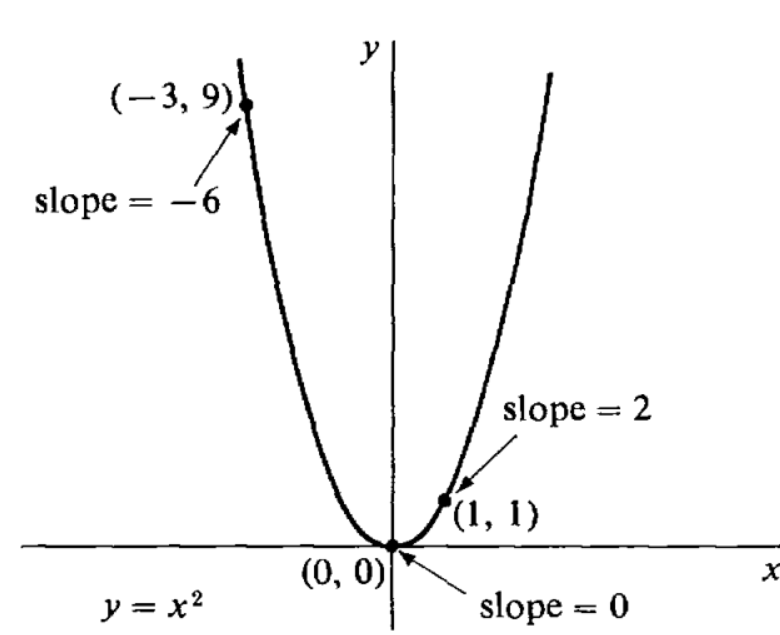
\includegraphics[width=.5\textwidth]{images/slope-examples-parabola}\end{figure}
\pause\item For Example, The Slope Is $2x_0=2\cdot 0=0$ at $(0,0)$, $2\cdot 1=2$ at $(1,1)$, And $2\cdot -3=-6$ at $(-3, 9)$.
\end{itemize}
\end{frame}

\begin{frame}
\frametitle{Introductory Calculus--Infinitesimal Approach}
\framesubtitle{1.4 Slope And Velocity; The Hyperreal Line 03}
\label{slide:1.4-03}
\begin{itemize}
\item We Can Visualize \alert{Slope as Velocity}.
\pause\item If The Horizontal Axis Represents Time And Vertical Axis Position, Is \alert{The Average Velocity between $(y_0,t_0)$ and $(y_0+\Delta y, t_0+\Delta t)$} = \alert{The Velocity \textit{at\footnote{In Physics, We Call It The \textit{Instantaneous Velocity}.}} Either} of Those Points?  
\pause\item Since in This Case The Velocity Constantly Increases, The Answer Is \alert{NO}.
\pause\item $v_{ave}=2t_0+\Delta t$ And, \alert{After We Treat $\Delta t$ Negligible}, $v_{ave}=2t_0$. 
\end{itemize}
\end{frame}

\begin{frame}
\frametitle{Introductory Calculus--Infinitesimal Approach}
\framesubtitle{1.4 Slope And Velocity; The \alert{Trouble with Intuition}}
\label{slide:1.4-04}
\begin{itemize}
\item In Either Case (Slope, Velocity), The Intuitive Reasoning Fails to Clarify \alert{When Something Is to Be Treated Negligible}.
\pause\item We Need a \alert{Sharp Distinction} between \alert{Which Numbers Are Small Enough to Ignore And Which Aren't}.
\pause\item Actually, \alert{No \underline{Real Number} Except $0$ Is Small Enough To Ignore\footnote{Does This Hint at a New \textit{Kind} of Number?}}.
\pause\item To Address This Difficulty, We \alert{Take The Bold Step\footnote{A Rigorous Treatment Is Provided by Keisler in His \textit{Foundations}.} of Introducing a New \textit{Kind\footnote{Unreal?} of Number}} Which Is \alert{Infinitely Small And Yet $\ne 0$}.
\end{itemize}
\end{frame}

\begin{frame}
\frametitle{Introductory Calculus--Infinitesimal Approach}
\framesubtitle{1.4 Properties of Infinitesimals}
\label{slide:1.4-05}
\begin{definition}[Infinitely Small Or Infinitesimal Number]
A \textit{Number} $\varepsilon$ Is Said to Be \textit{Infinitely Small, Or Infinitesimal,} If $-a<\varepsilon<a \quad\forall a\in\mathbb{R}^+$.
\end{definition}
\begin{itemize}
\item Note: All Infinitesimal Numbers Exist Between \textit{Every} Positive Real Number And Its Negative\footnote{M. Gardner Calls It The \textit{Number Neverland.}}.
\pause\item The \alert{Only \underline{Real} Infinitesimal Number is $0$}.
\pause\item We Introduce A New Number System, \alert{The Hyperreal Numbers}, Which \alert{Contains All The Real Numbers And \underline{Infinitesimals That Are Not Zero}}.
\pause\item \alert{Integers Create Rationals. Rationals Create Reals. Reals Create Hyperreals.}
\pause\item Right Now, \alert{We Study Properties of Hyperreals Needed for The Calculus}. We'll Study Their Creation Later.
\end{itemize}
\end{frame}

\begin{frame}
\frametitle{Introductory Calculus--Infinitesimal Approach}
\framesubtitle{1.4 Properties of Hyperreals And Infinitesimals}
\label{slide:1.4-06}
\begin{itemize}
\item $\mathbb{R}^*$: The Set of All Hyperreal Numbers.
\pause\item $x\in\mathbb{R}\implies x\in\mathbb{R}^*\implies\mathbb{R}\subseteq\mathbb{R}^*$. However, $\mathbb{R}^*$ Has Other Elements Too, \alert{$\therefore \mathbb{R}\subset\mathbb{R}^*$}.
\pause\item Infinitesimals in $\mathbb{R}^*$ Are of \alert{Three Kinds: Positive, Negative, And \underline{The Real Number $0$}}.
\pause\item $x,x_0,x_1,y,\dots$ Denote Reals. $\Delta x, \Delta y, \varepsilon\text{ (epsilon)},\delta\text{ (delta)},\dots$ Denote Infinitesimals.
\pause\item If $a,b\in\mathbb{R}^*$ And $a-b \text{ Is Infinitesimal}$, Then We Say \alert{$a$ Is ``Infinitely Close'' to $b$}.
\begin{itemize}
\pause\item If $\Delta x=(x_0+\Delta x)-(x_0)$ Is Infinitesimal, Then \alert{$x_0+\Delta x$ And $x_0$ Are ``Infinitely Close'' to Each Other}.
\end{itemize}
\pause \item If \alert{$\varepsilon$ Is Positive Infinitesimal}, Then 
\begin{itemize}
\pause\item\alert{$-\varepsilon$ Is Negative Infinitesimal}.
\pause\item\alert{$\frac{1}{\varepsilon}$ Is Infinite Positive, > All Real Numbers}.
\pause\item\alert{$\frac{-1}{\varepsilon}$ Is Infinite Negative, < All Real Numbers}.
\end{itemize}
\end{itemize}
\end{frame}

\begin{frame}
\frametitle{Introductory Calculus--Infinitesimal Approach}
\framesubtitle{1.4 More Properties of Hyperreals And Infinitesimals}
\label{slide:1.4-07}
\begin{itemize}
\item<1->
Hyperreal Numbers Which Are Not Infinite, Are \alert{Finite Numbers}.
\item<2->
About each $c\in\mathbb{R}$ Is \alert{A Portion of Hyperreal Line Composed of The Numbers Infinitely Close to $c$}.
\visible<2->
{
\begin{figure}[H]
\centering
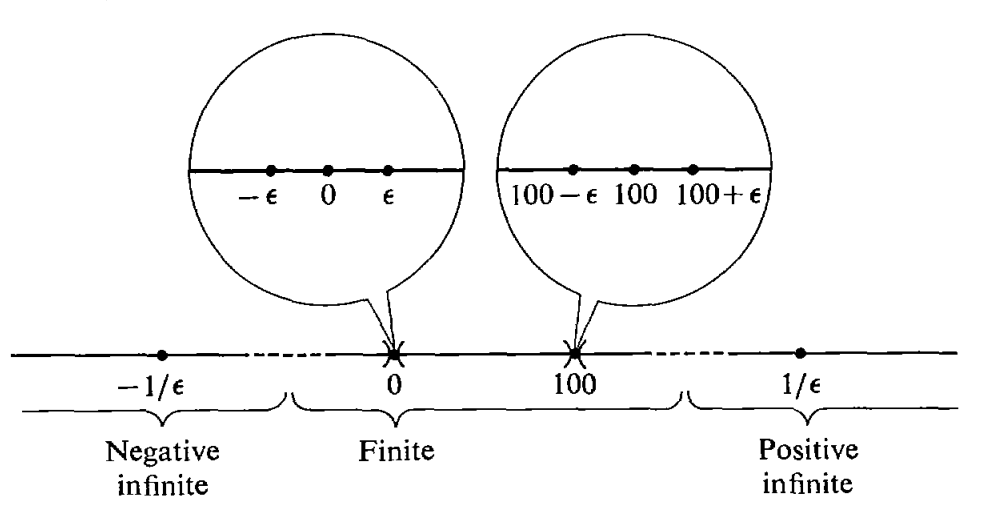
\includegraphics[width=.5\textwidth]{images/infinitesimal-microscope}
\caption{Finite And Infinite Parts of The Hyperreal Line (\textit{Infinitesimal Microscope} about $c=0,c=100$)}
\label{fig:finfinhyperreal}
\end{figure}
}
\item<3->
\alert{Numbers Infinitely Close to $0$ Are Infinitesimals}.
\end{itemize}
\end{frame}

\begin{frame}
\frametitle{Introductory Calculus--Infinitesimal Approach}
\framesubtitle{1.4 Startling Observation about \alert{The Physical Space}}
\label{slide:1.4-08}
\begin{block}{The Nature of Physical Space}
Euclid Struggled to Define \alert{a `Point': Something That Has a Position But No Magnitude\footnote{Isn't This `Definition' (\textit{Accepted} for Centuries) \textit{Meaningless}?}}.

We Have No Way of Knowing What a Line in Physical Space Is Really Like (``What Is It Composed of?''). It Might Be Like the Hyperreal Line (with Infinitesimals Surrounding Every `Real Point'), The Real Line (without Any Infinitesimals), Or Neither. \alert{However, in Applications of The Calculus It Is Helpful to Imagine a Line in Physical Space as A Hyperreal (Rather Than Real) Line. The Hyperreal Line Is, Like The Real Line, A Useful \underline{Mathematical Model}\footnote{And, Here's A Stark Reminder: All Models Are Wrong; Some Are Useful!} for A Line in Physical Space.}
\end{block}
\end{frame}

\begin{frame}
\frametitle{Introductory Calculus--Infinitesimal Approach}
\framesubtitle{1.4 Defining Slope w Infinitesimals}
\label{slide:1.4-09}
\begin{definition}[The \alert{Slope of A Curve at $(x_0,y_0)$}]

Let $y=f(x)$ Be a Certain Function. Let $P(x_0,y_0)$ Be Any Point on The Curve Representing $y$. \alert{Let $\Delta x$ Be a Positive Or Negative Infinitesimal}. Consider A Point $(x_0+\Delta x,y_0+\Delta y)$ \alert{Infinitely Close to P}.

Then,

\[
\text{Slope of $f$ at} (x_0,y_0)=\text{\alert{Real Number Infinitely Close to }} \frac{\Delta y}{\Delta x}
\]
\label{def:slope}
\end{definition}
Note: The Slope is \textit{Defined to Be} A Real Number.
\end{frame}

\begin{frame}
\frametitle{Introductory Calculus--Infinitesimal Approach}
\framesubtitle{1.4 Calculating Slopes with Infinitesimals: Examples}
\label{slide:1.4-10}
\begin{example}[Slope of $y=x^2$]
The Definition [\ref{def:slope}] Defines Slope as \alert{The Real Number Infinitely Close to $\frac{\Delta y}{\Delta x}$}.

\begin{equation}
\begin{aligned}
y+\Delta y &= (x+\Delta x)^2  \\
\therefore \Delta y &= 2x\Delta x+(\Delta x)^2 \\
\therefore \frac{\Delta y}{\Delta x} &= 2x+\Delta x \\
\therefore \text{Slope}&=2x \;\text{(From Definition [\ref{def:slope}])}
\end{aligned}
\label{eq:slope-of-y=x^2}
\end{equation}
\pause
$2x$ Is the \alert{Real Number Infinitely Close to The Hyperreal Number $2x+\Delta x$}.
\end{example}
\pause
In This Example It Was Rather Straightforward to Show $2x+\Delta x$ And $2x$ Are Infinitely Close To Each Other. 
\end{frame}

\begin{frame}
\frametitle{Introductory Calculus--Infinitesimal Approach}
\framesubtitle{1.4 Calculating Slopes with Infinitesimals: Examples}
\label{slide:1.4-11}
\begin{example}[Slope of $y=x^3$]
The Definition [\ref{def:slope}] Defines Slope as \alert{The Real Number Infinitely Close to $\frac{\Delta y}{\Delta x}$}.

\begin{equation}
\begin{aligned}
y+\Delta y &= (x+\Delta x)^3  \\
\therefore \Delta y &= \cancel{x^3}+3x^2\Delta x+3x(\Delta x)^2+(\Delta x)^3-\cancel{x^3}\\
\therefore \frac{\Delta y}{\Delta x} &= 3x^2+3x\Delta x+(\Delta x)^2 \\
\end{aligned}
\label{eq:slope-of-y=x^3}
\end{equation}
If (Because $\Delta x$ Is Infinitesimal), $3x\Delta x+(\Delta x)^2$ Is Infinitesimal, Then 
\begin{equation}
\begin{aligned}
\text{Slope}&=3x^2
\end{aligned}
\end{equation}
\end{example}
\end{frame}

\begin{frame}
\frametitle{Introductory Calculus--Infinitesimal Approach}
\framesubtitle{1.4 Which Hyperreal Numbers Are Infinitely Close to Each Other?}
\label{slide:1.4-12}
\begin{itemize}
\item
\alert{$\Delta x$ Is An Infinitesimal. That Brings $x+\Delta x$ Infinitely Close to $x$.}

\pause \item However, It Is Not Immediately Clear That $3x^2+3x\Delta x+(\Delta x)^2$ Is Infinitely Close to $3x^2$, Is It?
\pause \item It Depends on Whether $3x\Delta x+(\Delta x)^2$ Is Infinitesimal. We Only Know $\Delta x$ to Be Infinitesimal. Does That Make $3x^2+3x\Delta x+(\Delta x)^2$ Infinitesimal?

\pause\item Thus, Unless We Have Precise Rules To Determine Which Hyperreal Numbers Are \alert{Infinitely Close} to Which Real Numbers, We Won't Be Able to Go Too Far.
\end{itemize}
\pause
\alert{That's What We Study Next}.
\end{frame}

\begin{frame}
\frametitle{Introductory Calculus--Infinitesimal Approach}
\framesubtitle{1.5 Computations with Hyperreal Numbers}
\label{slide:1.5-01}
\begin{itemize}
\item Our Choice of The Mathematical Model of A Line in The Physical Space, \alert{The Hyperreal Line}, Contains Points Representing Real And Hyperreal Numbers.
\item Surrounding Each Real Number $r\in\mathbb{R}$, There Are \alert{Hyperreal Numbers Infinitely Close to $r$}.
\item Hyperreal Numbers Infinitely Close to 0 Are Called Infinitesimals.
\item $0$ Is The Only \textit{Real} Infinitesimal Number. There Are Many Nonzero Hyperreal Infinitesimals.
\pause\item In This Section, \alert{We Describe Hyperreal Numbers More Precisely And Develop a Facility for Computation with Them}.
\pause\item We Must Undertake This Effort, Because, After All, We Took \alert{The Bold Step of Conceiving \textit{Hyperreal Number: A New Kind of Number}}; We Must Follow Through!
\end{itemize}
\end{frame}

\begin{frame}
\frametitle{Introductory Calculus--Infinitesimal Approach}
\framesubtitle{1.5 Computations with Hyperreal Numbers}
\label{slide:1.5-02}
\begin{itemize}
\item In Our Quest, We Must Satisfactorily (Firmly, Rigorously) Answer Questions Such as:
\begin{itemize}
\pause\item $\Delta x$ Denotes An Infinitesimal. Do Familiar Functions (e.g. Polynomial, Rational, \dots) Map Infinitesimals on to Infinitesimals? Thus, If $\Delta x$ Infinitesimal, Is A Polynomial Function of Infinitesimals Alone, e.g. $(\Delta x)^2 -(\Delta x)$, Infinitesimal Too?
\pause\item How Do We Think of Functions That \alert{\textit{Combine} Infinitesimals with Reals}? For Example, \alert{Given That $\Delta x$ Is Infinitesimal, Is $\underline{2x\Delta x}+(\Delta x)^2$ Infinitesimal Too}?
\end{itemize}
\end{itemize}
\pause
Shouldn't We Get The Taste of The Pain That Robinson et.al. Had While Conceiving A New Kind of Number (Hyperreal) That Must Live Amicably with The Kind of Number (Real) That Already Existed And Was Widely Understood? 
\end{frame}

\begin{frame}
\frametitle{Introductory Calculus--Infinitesimal Approach}
\framesubtitle{1.5 Why `Resurrect' Infinitesimals?}
\label{slide:1.5-03}
What might Have inspired Robinson to take the effort?

Humans look at the historical context of developments. We rejoice in history. We respect those who came before us. After Karl Weierstrass `banished' infinitesimals with his rigorous reformulation of calculus (he also must have felt the burden of creation while conceiving ``this baby'' in the 1870s; he defied Newton, Euler, \dots), mathematical community thought that calculus was `solved'.

Why would Abraham Robinson, a young mathematician in the 1940s and 50s, ``bring infinitesimals back''? Did he want to become famous? Could he not banish infinitesimals convincingly? Why conceive a new kind of number and put it on a rigorous pedestal? Why solve a ``solved problem''?

These questions on ``Foundations of Mathematics'' are deep.
\end{frame}


\begin{frame}
\frametitle{Introductory Calculus--Infinitesimal Approach}
\framesubtitle{1.5 More: Why `Resurrect' Infinitesimals?}
\label{slide:1.5-04}
I haven't read sufficiently about Robinson's inspiration to conceive hyperreal numbers. 

However, my rather mundane opinion on this is that, after all, infinitesimals had been practically successful. Many brilliant mathematicians used them to solve practical problems before Weierstrass's reformulation of calculus. What was missing was the rigor. Perhaps Robinson felt dearly about providing a rigorous treatment to something that worked effectively. That became his life's work.

We don't want to get completely lost in questions like ``Is Mathematics Invented or Discovered?'', but can we ignore them?

\alert{Alright, Back to Answering Questions on Slide [\ref{slide:1.5-02}]: Computing with Hyperreals}.
\end{frame}

\begin{frame}
\frametitle{Introductory Calculus--Infinitesimal Approach}
\framesubtitle{1.5 The Extension Principle: Creating Hyperreals, Dealing with Real, Hyperreal Functions}
\label{slide:1.5-05}
\begin{itemize}
\item We Start with \alert{The Extension Principle}, Which \alert{Gives Us Hyperreal Numbers}, And \alert{Extends All Real Functions to Them}.
\pause
\item $f:\mathbb{R}\rightarrow\mathbb{R}$ Defines a \alert{Real-Valued Function}. When We Say $f(a)=b$, $f$ \textit{relates} Some $a\in\mathbb{R}$ to Some $b\in\mathbb{R}$. $f$ May Fail to Relate some $a\in\mathbb{R}$ with Any Real Number. Then We Say $f(a)$ is \textit{Undefined}.
\pause\item Similarly, $F$, \alert{A Hyperreal Function}, \textit{relates} A Hyperreal Number $H$ with Another Hyperreal Number $K$, Or Is \textit{Undefined}. Symbolically, $F:\mathbb{R}^*\rightarrow\mathbb{R}^*$. We say $K=F(H)$.
\pause\item We Can, Like Real-Valued Functions, Easily Define Hyperreal Functions of More Than 1 Hyperreal Number.
\end{itemize}
\end{frame}

\begin{frame}
\frametitle{Introductory Calculus--Infinitesimal Approach}
\framesubtitle{1.5 The Extension Principle: Three Parts}
\label{slide:1.5-06}
\begin{itemize}
\item a) $\mathbb{R}\subset\mathbb{R}^*$. The Order Relation `$<$' for $\mathbb{R}$ Is A Subset of The Order Relation `<' for $\mathbb{R}^*$. This Part Asserts That \alert{The Real Line \textit{Is A Part of} The Hyperreal Line}.
\pause\item b) \alert{There's A Hyperreal Number Greater Than Zero But Less Than Every Positive Real Number}. This Part Begets A Precise Definition of Infinitesimals.
\pause\item c) For Every $f:\mathbb{R}\rightarrow\mathbb{R}$ (of One Or More Variables), We Are Given \alert{A Hyperreal Function, $f^*$, Called The \textit{Natural Extension of $f$}}. This Part Allows Us to Apply Real Functions to Hyperreal Numbers.
\end{itemize}
\end{frame}

\begin{frame}
\frametitle{Introductory Calculus--Infinitesimal Approach}
\framesubtitle{1.5 The Extension Principle Part b) Precise Definition of \alert{\textit{Infinitesimal}}}
\label{slide:1.5-07}
Restating Part b):
\begin{itemize}
\item \alert{There's A Hyperreal Number Greater Than Zero But Less Than Every Positive Real Number}. This Part Begets A Precise Definition of Infinitesimals.
\end{itemize}
\begin{definition}[Infinitesimal]
A Hyperreal Number $b$ Is Said To Be \alert{Positive Infinitesimal} If $b>0$, But Less Than Every Positive Real Number. \\
A Hyperreal Number $b$ Is Said To Be \alert{Negative Infinitesimal} If $b<0$, But Greater Than Every Negative Real Number. \\
A Hyperreal Number $b$ Is Said To Be \alert{Infinitesimal} If It Is \alert{Either Positive Infinitesimal, Negative Infinitesimal, Or Zero}.
\label{def:infinitesimal}
\end{definition}
\end{frame}

\begin{frame}
\frametitle{Introductory Calculus--Infinitesimal Approach}
\framesubtitle{1.5 The Extension Principle Part c) Extending Real Functions}
\label{slide:1.5-08}
\begin{itemize}
\item We \alert{\textit{Naturally} Extend Real-Valued Functions to Functions That Operate on Hyperreal Numbers}.
\begin{itemize}
\pause\item For Example, \alert{If $x,y$ Are Hyperreal Numbers, $x+y$ Adds Them Just Like $+$ Adds Two Real Numbers}.
\pause\item \alert{If $x,y$ Are Hyperreal Numbers, A \textit{Real Expression} Such as $\sin(x+\cos(y))$ Implies Natural Extensions of the $\sin,\cos$ Functions to Them}.
\end{itemize}
\end{itemize}
\end{frame}

\begin{frame}
\frametitle{Introductory Calculus--Infinitesimal Approach}
\framesubtitle{1.5 The Transfer Principle}
\label{slide:1.5-09}
\begin{definition}[Transfer Principle]
Every \alert{Real Statement} That Holds for One Or More Particular Real Functions Holds for The Hyperreal Natural Extensions of These Functions.
\label{def:transfer-principle}
\end{definition}
\end{frame}

\begin{frame}
\frametitle{Introductory Calculus--Infinitesimal Approach}
\framesubtitle{1.5 Examples of \alert{\textit{Real Statements}}}
\label{slide:1.5-10}
\begin{example}[Real Statements]
\label{ex:real-statements}
If $x,y$ Are Real Numbers, The Following Hold:
\begin{enumerate}
\item Closure Law of Addition: $x+y$ Is Defined.
\item Commutative Law of Addition: $x+y=y+x$.
\item A Rule for Order: If $0<x<y$, Then $0<\frac{1}{y}<\frac{1}{x}$.
\item Division by Zero ($\frac{x}{0}\;\text{or}\;\frac{0}{0}$) Is Undefined.
\item An Algebraic Identity: $(x-y)^2=x^2-2xy+y^2$. 
\item A Trigonometric Identity: $\sin^2x+\cos^2x=1$.
\item A Rule for Logarithms: If $x>0,y>0$, Then $\log xy=\log x + \log y$.
\end{enumerate}
\end{example}
The Transfer Principle States That These \alert{Statements @ Sophisticated Real-Valued Functions Also Hold When We Apply Them to Hyperreal Numbers}.
\end{frame}

\begin{frame}
\frametitle{Introductory Calculus--Infinitesimal Approach}
\framesubtitle{1.5 More Examples of \alert{\textit{Real Statements}}}
\label{slide:1.5-11}
\begin{example}[More Real Statements]
\label{ex:more-real-statements}
If $x,y$ Are Real Numbers, The Following Hold:
\begin{enumerate}
\item The Square-root Function: $y=\sqrt{x} \iff y^2=x\;\text{and}\;x\geq 0$.
\item The Absolute Value Function: $y=\mid x\mid\iff y=\sqrt{x^2}$.
\item The Common Logarithm Function: $y=\log_{10} x\iff 10^y=x$.
\end{enumerate}
\end{example}
\alert{The Transfer Principle States That The Natural Extensions of These Functions Hold for Hyperreal Numbers}.
\end{frame}

\begin{frame}
\frametitle{Introductory Calculus--Infinitesimal Approach}
\framesubtitle{1.5 Using Extension And Transfer Principles for Hyperreal Computations}
\label{slide:1.5-12}
We Now Logically Proceed to Doing Computations Involving Hyperreal Numbers.
\begin{itemize}
\item The Extension Principle Tells Us That At Least One Positive Infinitesimal, $\varepsilon$, Exists. By Definition, $\varepsilon$ Is \textit{Infinitely Close to 0}.
\pause\item Readily, The Transfer Principle Suggests $0<\varepsilon^2<\varepsilon$ (Follows from the `Real Statement': $0<r^2<r\;\forall r\in\mathbb{R}^+\mid 0<r<1$).
\pause\item It Follows That We Can Now Construct Infinitely Many Infinitesimals. Here Are Some Examples Listed In An Order of Increasing Magnitude: $\varepsilon^3,\varepsilon^2,\frac{\varepsilon}{100},\varepsilon,75\varepsilon,\sqrt{\varepsilon},\varepsilon+\sqrt{\varepsilon}$.
\end{itemize}
\end{frame}

\begin{frame}
\frametitle{Introductory Calculus--Infinitesimal Approach}
\framesubtitle{1.5 A Parallel Definition}
\label{slide:1.5-13}
We Defined \alert{Infinitesimal} in Definition [\ref{def:infinitesimal}].

We Have a Corresponding Definition Pertaining The Other Hyperreal Numbers.
\begin{definition}[Finite And Infinite Hyperreal Number]
A Hyperreal Number $b$ Is
\begin{enumerate}
\item \alert{\textit{Finite}}, If $b$ Is between Two Real Numbers.
\item \alert{\textit{Positive Infinite}} If $b$ Is Greater Than Every Real Number.
\item \alert{\textit{Negative Infinite}} If $b$ Is Less Than Every Real Number.
\end{enumerate}
\label{def:finite-infinite}
\end{definition}
Since Every \alert{Infinitesimal} Is between $0$ And, Say, $1$ (Which Are Both Real Numbers), It Is \alert{Finite}. Clearly, \alert{Not Every Finite Is Infinitesimal}.
\end{frame}

\begin{frame}
\frametitle{Introductory Calculus--Infinitesimal Approach}
\framesubtitle{1.5 Ready for Rules of Hyperreal Computations}
\label{slide:1.5-14}
Now That The Definitions of Real Numbers And Infinitesimal [\ref{def:infinitesimal}], Finite, And Infinite Hyperreal Numbers [\ref{def:finite-infinite}] Are Established, We Are Ready for Rules for Their Computations. These Rules, Which Are Intuitive, Can Be Rigorously Proved{\footnote{\alert{TBD!}}} From Those Definitions Using Standard Proof Techniques.
\begin{definition}[Denoting Hyperreal Numbers of Various Kinds]
We Assume The Following:
\begin{enumerate}
\item \alert{$\varepsilon,\delta$ Are Infinitesimal}.
\item \alert{$b,c$ Are Finite But Not Infinitesimal}.
\item \alert{$H,K$ Are Infinite}.
\end{enumerate}
\end{definition}
\end{frame}

\begin{frame}
\frametitle{Introductory Calculus--Infinitesimal Approach}
\framesubtitle{Rules for Hyperreal Computations: Real Numbers}
\label{slide:1.5-15}
\begin{hyperrule}[Real Numbers]
\begin{enumerate}
\item $0$ Is The Only Real Infinitesimal Number.
\item Every Real Number is Finite.
\end{enumerate}
\end{hyperrule}
\end{frame}

\begin{frame}
\frametitle{Introductory Calculus--Infinitesimal Approach}
\framesubtitle{Rules for Hyperreal Computations: Negatives}
\label{slide:1.5-16}
\begin{hyperrule}[Negatives]
\begin{enumerate}
\item $-\varepsilon$ Is Infinitesimal.
\item $-b$ Is Finite But Not Infinitesimal.
\item $-H$ Is Infinite.
\end{enumerate}
\end{hyperrule}
\end{frame}

\begin{frame}
\frametitle{Introductory Calculus--Infinitesimal Approach}
\framesubtitle{Rules for Hyperreal Computations: Reciprocals}
\label{slide:1.5-17}
\begin{hyperrule}[Reciprocals]
\begin{enumerate}
\item $\frac{1}{\varepsilon}$ Is Infinite.
\item $\frac{1}{b}$ Is Finite But Not Infinitesimal.
\item $\frac{1}{H}$ Is Infinitesimal.
\end{enumerate}
\end{hyperrule}
\end{frame}

\begin{frame}
\frametitle{Introductory Calculus--Infinitesimal Approach}
\framesubtitle{Rules for Hyperreal Computations: Sums}
\label{slide:1.5-18}
\begin{hyperrule}[Sums]
\begin{enumerate}
\item Addition of Hyperreal Numbers Is Commutative (Extension Principle).
\item $\varepsilon+\delta$ Is Infinitesimal.
\item $\varepsilon+b$ Is Finite But Not Infinitesimal.
\item $\varepsilon+H$ Is Infinite.
\item $b+c$ Is Finite (Could Be Infinitesimal Because $c$ May Be $-b+\varepsilon$).
\item $b+H$ Is Infinite.
\item \alert{$H+K$ Is Indeterminate}.
\end{enumerate}
\end{hyperrule}
\end{frame}

\section{Chapter 2}
\section{Summary}

\end{document}


